% journal_discussion.tex — Sections 6-8 of the journal manuscript.

\section{Discussion}
\subsection{Relation to the earlier analysis}
\label{sec:earlier}
The earlier analysis made five claims. Three are withdrawn or revised. The
catastrophic GP failure on large domains is a kernel-specification artefact:
with the amplitude estimated, the GP no longer reverts to the mean
(Fig.~\ref{fig:dom}). The spectral acquisition criterion gives no advantage
over plain committee variance on any of the six models on which it was
tested, and is worse on three. The committee's advantage is not general but
comes from a member that matches the dominant term, which a GP with a
quadratic trend or a sparse PCE reproduces on its own. Two claims survive:
aggregation must be error-weighted, and an adaptive committee can be more
accurate than a passive one: it was on four of the seven models on which it
was run, including the CFD case, although it remained less accurate than
the log-variable GP wherever the output is positive, and its exceedance
probabilities were worse on the plume and CFD cases. The records of the earlier
campaigns are kept in the repository~\repocite.

\begin{figure}[tb]
\centering
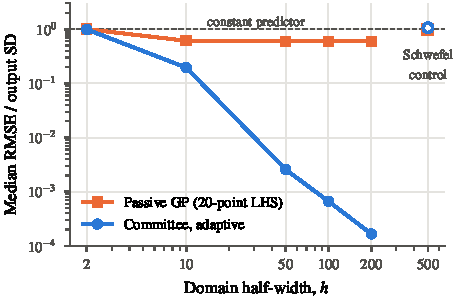
\includegraphics[width=0.62\textwidth]{fig_domain_sweep}
\caption{Physics model on $[-h,h]^3$, $N=20$: median nRMSE over 30 seeds
against the domain half-width, for the GP with the original kernel
(amplitude fixed), the Mat\'ern ARD GP with amplitude, and the committee of
the earlier analysis. Open markers: Schwefel function on $[-500,500]^3$.
Dashed line: constant predictor.}
\label{fig:dom}
\end{figure}

\subsection{What the surrogate contribution should be}
The coverage results separate two uses of a surrogate's uncertainty.
Pointwise, the GP posterior is a useful but uncalibrated description: it
locates where the surrogate is uncertain, which is why it drives good
adaptive designs at larger budgets, but its scale is set by a covariance
model fitted to 20 runs and is too small wherever that model is wrong. For
an uncertainty statement the scale is what matters, and the leave-one-out
residuals estimate it directly, without trusting the covariance model; the
jackknife+ turns them into intervals with a guarantee. The difference is
largest for the reported quantities. A GUM~S1 coverage interval of $Y$ is
fairly robust, because surrogate error that varies across the input space
partly averages out in the distribution of $Y$, and adding the LOO error
to each trial restores its nominal coverage. A 95th percentile or an
exceedance probability is not robust: it depends on the surrogate in a
small region. Intervals from the GP posterior contained the true value in
a median 63\% of the seeds (median over model and surrogate), whereas the
jackknife over LOO fits did so in a median 97\%. Integrating out the
hyperparameters narrowed this gap but did not close it
(Section~\ref{sec:res-robust}): the shortfall comes from covariance models
that do not fit the response, not only from plug-in estimates, and a
Bayesian treatment inherits the covariance model. Rescaling the GP SD by the
LOO standardised residuals, which keeps the GP's localisation of the error
and takes its scale from the runs, came closer, but the jackknife remained
the more reliable description. We therefore recommend the LOO error as the
surrogate contribution, and the jackknife over LOO fits for the uncertainty
of quantities derived from the propagated distribution.

\subsection{Limitations}
The study covers twelve models with up to 20 inputs and budgets of 10 to
80 runs; problems with many more inputs, where sparse and additive
structures matter more, may rank the surrogates differently. Two models were run with
a single budget per input distribution, and the adaptive committees were
run only up to $N=40$ because of their cost. The CFD case is
two-dimensional and steady, with a standard $k$--$\varepsilon$ model; it is a
benchmark with the features a dispersion simulation has, not a validated
prediction for a site, and its reference distribution is built from 800
runs rather than $2\times10^5$. The coverage results are averages over
seeds; for single designs the GUM~S1 interval fell below 90\% in at most
10\% of the designs of a model at $N=20$, and the jackknife+ guarantee (at
least 90\% for nominal 95\%) holds on average over designs, not for every
design. The LOO residuals describe only the errors that the runs can
reveal: a local feature that no run hits goes unnoticed
(Section~\ref{sec:res-robust}), and an error at the level of the
observation noise, shared by all LOO fits, is not seen by the jackknife.
The hyperparameter search ranges were fixed in advance; on the physics
model the amplitude reached the upper end of its range, which understates
the GP there (Section~\ref{sec:res-main}). Several output quantities were
studied on one model only; there, resampling the LOO residual vectors run
by run, which preserves their correlation, gave the nominal coverage of the
GUM~S2 region~\cite{jcgm102}, and resampling the components independently
over-stated the region. The log transformation applies only to positive
outputs, and its back-transformation to the predictive median slightly
underestimates the mean of a skewed output; the bias is included in the
validation errors reported. Finally, the paired tests are exploratory: all
$p$-values were Holm-adjusted together, and nominal differences that do not
survive the adjustment are not claimed.

\section{A procedure for surrogate-based GUM~S1 evaluations}
\label{sec:procedure}
Fig.~\ref{fig:flowchart} condenses the results into a procedure that needs
only the $N$ runs. Its two key steps were validated on the twelve models: the
selection of the surrogate by its LOO error recovered practically all the
benefit of the best specification (Section~\ref{sec:res-select}), and the
LOO error as surrogate contribution restored the nominal coverage of the
GUM~S1 coverage interval (Section~\ref{sec:res-coverage}). Candidates should
include a GP with an estimated amplitude, one length scale per input and a
quadratic trend, and a sparse PCE, each on the log scale when the output
is positive; a fitted hyperparameter at the end of its search range is a
sign that the range should be widened. With fewer than 19 runs a 95\%
jackknife+ interval is unbounded, but the GUM~S1 coverage interval with the
LOO residuals remained valid down to ten runs. The LOO error covers what the
runs can reveal: where a narrow feature is plausible (a narrow plume, a
local flow structure), prior knowledge or runs placed there are needed.
Adaptive designs are optional: a targeted design such as
AK-MCS is worthwhile when a threshold decision is the purpose and the
threshold lies in a tail of the distribution, and
variance-driven designs when the budget is several times the number of
inputs and the model is smooth.

\begin{figure}[tb]
\centering
% fig_flowchart.tex — decision procedure for surrogate-based GUM S1
% propagation (Section "Practical procedure"). \input inside a figure;
% needs \usetikzlibrary{positioning,arrows.meta,shapes.geometric}.
\begin{tikzpicture}[
  node distance=3.2mm and 6mm,
  box/.style={draw, rounded corners=1.5pt, align=center, font=\footnotesize,
              text width=#1, inner sep=2.5pt, fill=white},
  box/.default=54mm,
  dec/.style={draw, diamond, aspect=2.6, align=center, font=\footnotesize,
              inner sep=0.5pt, fill=gray!8},
  side/.style={draw, dashed, rounded corners=1.5pt, align=left, font=\scriptsize,
               text width=30mm, inner sep=2pt},
  arr/.style={-{Latex[length=1.6mm]}, semithick},
  lab/.style={font=\scriptsize}]
\node[box] (start) {Model $Y=f(\mathbf X)$ too costly for $10^5$ Monte Carlo
  trials; budget of $N$ runs};
\node[box, below=of start] (design) {Run $f$ on an $N$-point Latin hypercube
  drawn in the input distribution (inverse-CDF map)};
\node[dec, below=of design] (pos) {$Y>0$, multiplicative?};
\node[box, below=of pos] (fit) {Fit candidates on the log scale if \emph{yes}:
  GP (Mat\'ern-5/2, ARD, estimated amplitude, nugget; $\pm$ quadratic
  trend) and sparse PCE (LAR, corrected LOO); no hyperparameter at the
  end of its search range};
\node[box, below=of fit] (sel) {Keep the candidate with the smallest
  leave-one-out (LOO) error};
\node[dec, below=of sel] (ok) {LOO error fit\\for purpose?};
\node[box, below=of ok] (prop) {GUM S1 propagation through the surrogate,
  adding to every trial a draw of the LOO residuals};
\node[box, below=of prop] (rep) {Report $y$, $u(y)$ and the coverage
  interval (trials by GUM S1 7.9); state the surrogate contribution;
  intervals for derived quantities by the jackknife over the LOO fits};
\node[side, right=of ok] (more) {Add runs, e.g.\ while the surrogate
  share of $u^2(y)$ exceeds 1\%: extend the design (space filling); a
  targeted design only for a threshold decision};
\node[side, right=of prop] (no) {Not the GP posterior SD, nor a committee
  envelope: both understate the surrogate error};
\draw[arr] (start) -- (design);
\draw[arr] (design) -- (pos);
\draw[arr] (pos) -- (fit);
\draw[arr] (fit) -- (sel);
\draw[arr] (sel) -- (ok);
\draw[arr] (ok) -- node[lab, right] {yes} (prop);
\draw[arr] (prop) -- (rep);
\draw[arr] (ok) -- node[lab, above] {no} (more);
\draw[arr] (more.north) |- (design.east);
\draw[dashed] (no.west) -- (prop.east);
\end{tikzpicture}

\caption{Procedure for a GUM~S1 evaluation with a surrogate fitted to $N$
runs of an expensive model.}
\label{fig:flowchart}
\end{figure}

\subsection{Worked example}
\label{sec:worked}
The procedure is implemented in \texttt{src/procedure.py} of the
repository~\repocite; given the $N$ runs and a sampler of the input
distribution, it returns the GUM~S1 results with and without the surrogate
contribution, jackknife intervals of the reported quantities and an
uncertainty budget. The number of Monte Carlo trials is chosen by the
adaptive procedure of GUM~S1~\cite{jcgm101} (clause 7.9) for a stated number
of significant digits of $u(y)$. Applied to the CFD case with the 20 runs
of the first design, it chose the log-scale GP with a quadratic trend, whose LOO RMSE (23\,mg\,m$^{-3}$) was smaller than those of the
log-scale GP (31), the log-scale sparse PCE (93) and the raw-scale
candidates (157--260). Two significant digits of $u(y)$ (numerical
tolerance 5\,mg\,m$^{-3}$) took 115 batches of $10^4$ trials, $M=1.15\times10^6$;
the upper limit of the coverage interval was the last quantity to settle.
Table~\ref{tab:worked} compares the result with the reference, which a
practitioner would not have. Adding the LOO residuals changed the reported
quantities by at most 1.3\%; here it lowered them,
because the residuals have a negative mean ($-0.013$ on the log scale,
mostly from one run). The reported 95\% coverage interval contains
94.3\% of the reference distribution. The jackknife intervals, which
describe the surrogate error alone, contain the reference values of the
mean, the lower limit of the coverage interval and $P(C>\mathrm{IDLH})$;
for the SD, the 95th percentile and the upper limit the reference lies
0.7--1.6\% above the upper end of the interval, by less than half the
standard uncertainty of the reference itself.

The GUM uncertainty framework, the law of propagation of uncertainty applied
to the same surrogate at the input means, gives $y=318$\,mg\,m$^{-3}$,
$u(y)=232$\,mg\,m$^{-3}$ and the interval $y\pm1.96\,u(y)=[-137,772]$\,mg\,m$^{-3}$,
which contains only 85.5\% of the reference distribution and extends to
impossible negative concentrations. For this skewed output the Monte Carlo
method of GUM~S1, and therefore a surrogate, is needed.

The budget treats the surrogate error $E$ as one more input quantity of
the model~\eqref{eq:contrib}, with $E$ drawn from the LOO residuals, and gives first-order variance shares of the inputs and the
total share of $E$ (estimators of Saltelli et al.~\cite{saltelli2010}).
The reference wind speed contributed 36\% of $\mathrm{Var}(Y)$, the release
rate 29\%, the receptor distance 5.9\%, the turbulent Schmidt number 4.2\%,
the building height 3.2\% and the roughness length 1.7\%; interactions
between the inputs 20\% and the surrogate 0.3\%. With this surrogate, then,
the evaluation is limited by the input uncertainties rather than by the
number of runs, and further CFD runs would mainly narrow the jackknife
intervals of the tail quantities. The budget is how a practitioner can
tell whether more runs are worth their cost: a surrogate share comparable
to those of the inputs would indicate the opposite.

\begin{table}[tb]
\centering
\caption{Worked example: the procedure of Fig.~\ref{fig:flowchart} on the
CFD case with $N=20$ runs and $M=1.15\times10^6$ trials, chosen by the
adaptive procedure of GUM~S1 (mg\,m$^{-3}$). Columns:
surrogate treated as exact; with the LOO residuals added (the reported
result); 95\% jackknife interval over the LOO fits (surrogate error only);
reference from 800 CFD runs with its standard uncertainty in parentheses.}
\label{tab:worked}
\small
\begin{tabular}{l rr c r}
\toprule
Quantity & exact & with $E$ & jackknife & reference\\
\midrule
\tabinput{../results/journal/tab_worked.tex}
\bottomrule
\end{tabular}
\end{table}
